% ch-wetting.tex -- theory: disjoining pressure, contact angle, equilibrium drops, sizing
\chapter{Wetting and the contact line}
\label{ch:wetting}

The long-wave approximation assumes small slopes, and a contact line is the one
place in a thin film where the slope is not small. Yuzen handles it the way
lubrication models normally do: it never lets the thickness reach zero, keeps a
thin precursor film everywhere, and adds a disjoining pressure whose job is to
reproduce the correct equilibrium contact angle in the transition between the
precursor and the drop.

That device works, but it works only within limits, and the limits are
quantitative. This chapter derives the calibration, checks it analytically,
solves the equilibrium drop, and then shows the two things that decide whether
your case can deliver the contact angle you asked for: how thick the drop is
compared with the precursor, and how fine the mesh is compared with the
transition region. If you are setting up a wetting calculation, the last two
sections are the ones that will change what you type into the input file.

\section{The disjoining-pressure model and the calibration of \texorpdfstring{$\Dpn$}{Dp}}
\label{sec:wetting:dp}

In dimensional form the disjoining pressure is

\begin{equation}\label{eq:pi-dim}
  \Pi(h) = B \left[ (\hstar/h)^{n} - (\hstar/h)^{m} \right],
  \qquad n > m > 1,
\end{equation}

where $\hstar$ is the precursor thickness and the conventional exponent pair is
$(n,m) = (3,2)$. The first term is repulsive, the second attractive, and they
balance exactly at $h = \hstar$. That pair is the default of
\key{ExponentN} and \key{ExponentM}, whether the
\key{Physics.DisjoiningPressure} block is written without them or left out
(\cref{tab:physics-disjoining-keys}).

The coefficient $B$ is not free: it is fixed by requiring that the model
reproduce a chosen equilibrium contact angle $\thetae$. The condition is an
energy balance --- \emph{the difference in surface energy between the wetted
and the dry substrate equals the integral of the disjoining pressure across the
film} --- which reads

\begin{equation}\label{eq:energy-balance}
  \sigma\,(1 - \cos\thetae)
    = \frac{B\,\hstar\,(n-m)}{(n-1)(m-1)},
\end{equation}

and solving it for $B$ gives

\begin{equation}\label{eq:B-coef}
  B = \frac{(n-1)(m-1)}{\hstar\,(n-m)}\,\sigma\,(1 - \cos\thetae).
\end{equation}

In the long-wave regime $\thetae$ is small, so $1-\cos\thetae$ is replaced by
$\thetae^{2}/2$ --- an approximation whose error is tabulated exactly in
\cref{tab:cos-error}, and which is one of the reasons to keep the requested
angle small. Dividing \cref{eq:B-coef} by the pressure scale
$\sigma h_0 / L_0^{2}$ then produces the coefficient the code actually builds:

\begin{equation}\label{eq:dp-def}
  \Dpn = \frac{\As\,(n-1)(m-1)}{2\,\Hstar\,(n-m)}\;\thetae^{2}.
\end{equation}

Read \cref{eq:dp-def} as a statement about which knobs do what. The angle
\key{ContactAngle} moves $\Dpn$ as $\thetae^{2}$, so it is the key that sets
the wetting behavior. The other three --- \key{ExponentN}, \key{ExponentM} and
the precursor ratio $\Hstar$ --- also appear in \cref{eq:dp-def}, and they
appear there precisely so that their effect on the angle cancels.

\begin{note}[Changing the exponents or the precursor ratio does not change the target angle]
  $\Dpn$ is rebuilt from $n$, $m$ and $\Hstar$ every time, so the angle the
  model aims at stays exactly $\thetae$ whatever you do to them. What does
  change is the thickness of the precursor film and the width of the transition
  region between precursor and drop --- and therefore, as
  \cref{sec:wetting:apparent,sec:wetting:sizing} show, how much of the angle
  you actually get and how fine a mesh you need to see it.
\end{note}

\section{The analytic check}
\label{sec:wetting:analytic}

That \cref{eq:dp-def} really is consistent with the contact angle can be
verified exactly, without solving anything numerically. Take the limit in which
the precursor extends to infinity --- zero pressure, $K = 0$, and a far-field
thickness $\Hf = \Hstar$. The integral of the dimensionless disjoining pressure
over the whole film is elementary:

\begin{equation}\label{eq:pi-integral}
  \int_{\Hstar}^{\infty} \Pihat\,\mathrm{d}H
    = \frac{\Hstar\,(m-n)}{(n-1)(m-1)}.
\end{equation}

Feeding \cref{eq:pi-integral} into the first integral of the equilibrium
equation (\cref{sec:wetting:equilibrium}) gives the far-field slope of the
profile:

\begin{equation}\label{eq:slope-limit}
  (H')^{2} \;\longrightarrow\;
    \frac{2\,\Dpn\,\Hstar\,(n-m)}{(n-1)(m-1)} = \As\,\thetae^{2}.
\end{equation}

Now apply the conversion of \cref{eq:slope-conversion}. Since
$\As = (L_0/h_0)^{2} = 1/\varepsilon^{2}$, the dimensionless slope is
$H' = \thetae/\varepsilon$, and the physical slope $\varepsilon H'$ is
\emph{exactly} $\thetae$. The calibration is not approximate in this limit; it
is an identity. Everything that follows in this chapter is about how far a real
case sits from that limit.

\section{The equilibrium drop}
\label{sec:wetting:equilibrium}

Equilibrium means zero flux, which by \cref{eq:flux} means uniform pressure.
Keeping capillary and disjoining pressure only, in one dimension, that is

\begin{equation}\label{eq:eq-ode}
  H'' + \Dpn\,\Pihat(H) = K,
\end{equation}

with the constant $K$ equal to the (uniform) pressure. Multiplying
\cref{eq:eq-ode} by $H'$ and integrating once gives a first integral,

\begin{equation}\label{eq:first-integral}
  \tfrac{1}{2}\,(H')^{2}
    = K\,(H - \Hf) - \Dpn\,\bigl[\,W(H) - W(\Hf)\,\bigr],
  \qquad
  W(H) = \int_{\Hstar}^{H} \Pihat\,\mathrm{d}s .
\end{equation}

$\Hf$ is the flat film surrounding the drop. There $H' = H'' = 0$, so
\cref{eq:eq-ode} fixes the pressure,

\begin{equation}\label{eq:K-from-Hf}
  K = \Dpn\,\Pihat(\Hf).
\end{equation}

At the summit $H = \Hmax$ the slope vanishes too, so the right-hand side of
\cref{eq:first-integral} must be zero there:

\begin{equation}\label{eq:Hf-Hmax}
  K\,(\Hmax - \Hf) - \Dpn\,\bigl[\,W(\Hmax) - W(\Hf)\,\bigr] = 0 .
\end{equation}

\Cref{eq:Hf-Hmax} ties $\Hf$ to $\Hmax$: choose one and the other follows.
\textbf{Equilibrium drops are therefore a one-parameter family.} Fix $\Hmax$
and the entire shape is obtained by integrating a single ordinary differential
equation --- no partial differential equation, no time stepping, no iteration
on the whole field.

\file{tools/make\_equilibrium\_1d.py} does exactly this and writes the result
in the ASCII restart format, so an equilibrium drop can be used as an initial
condition or as a reference solution. It is the basis of the disjoining-pressure
verification in \cref{sec:verification:disjoining}.

\begin{figure}[tbp]
  \centering
  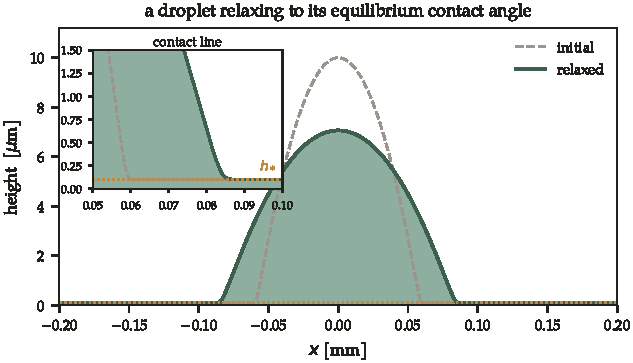
\includegraphics[width=0.85\textwidth]{../figures/wetting.pdf}
  \caption{A drop finding its equilibrium, from \file{wet\_static.toml} at
    $\thetae = \ang{10}$. The initial condition (dashed) is the equilibrium
    droplet of \ang{20}, \SI{10}{\micro\metre} high, on a precursor film of
    $\Hstar = 0.01$ (\SI{0.1}{\micro\metre}, dotted), resolved by
    $\Delta x = \SI{0.2}{\micro\metre}$; the solid curve is the free surface
    when the run has reached a steady state, at \SI{2.92}{\second}. The drop has
    spread to an apparent angle of \ang{9.71}, below $\thetae$ by the
    precursor bias of the next section, and the flat film around it settles
    \SI{0.5}{\percent} above $\Hstar$ ($\Hf$ of \cref{eq:Hf-Hmax}). The
    inset shows the contact line.\label{fig:wetting:relax}}
\end{figure}

\section{The apparent contact angle and the precursor bias}
\label{sec:wetting:apparent}

The equilibrium drop of a model with a \emph{finite} precursor does not show
the angle $\thetae$ unless $\Hmax/\Hstar$ is large. Outside the drop, where
disjoining pressure has died away, \cref{eq:eq-ode} reduces to $H'' = K$ and
the profile is a parabola. Extrapolating that parabola down to $H = 0$ and
reading its slope there is what corresponds to the angle measured
experimentally. It can be written in closed form:

\begin{equation}\label{eq:theta-cap}
  \thetacap = \varepsilon\,\sqrt{-2 K \Hmax}
            = \thetae \left( 1 - \frac{\Hstar}{2\Hmax} \right).
\end{equation}

\Cref{tab:apparent-angle} evaluates \cref{eq:theta-cap} for $\thetae = 10^\circ$
and $(n,m) = (3,2)$, alongside the largest slope the computed profile actually
attains anywhere.

\begin{yzntable}{Apparent angle and maximum profile slope, for $\thetae = 10^\circ$ and $(n,m)=(3,2)$\label{tab:apparent-angle}}{@{}d d d@{}}
\textsf{\bfseries $\Hmax/\Hstar$} & \textsf{\bfseries apparent angle [deg]} &
\textsf{\bfseries max.\ slope of the profile [deg]} \\ \midrule
2    & 7.5000 & 0.6320 \\
5    & 9.0000 & 3.6012 \\
10   & 9.5000 & 5.4236 \\
20   & 9.7500 & 6.7634 \\
50   & 9.9000 & 7.9627 \\
100  & 9.9500 & 8.5652 \\
1000 & 9.9950 & 9.5504 \\
\end{yzntable}

\begin{warn}[At $\Hmax/\Hstar = 2$ the model does not contain the angle you asked for]
  Read the first row. With a drop only twice as thick as its precursor, the
  apparent angle is $7.50^\circ$ and the steepest point of the profile is
  inclined at $0.63^\circ$. The $10^\circ$ that was written into
  \key{ContactAngle} is simply not present anywhere in the solution --- not as
  a measured value, not as a slope, not as an asymptote. This is not a
  discretization error and no mesh will remove it.

  Concretely: \textbf{a \SI{10}{\micro\metre} drop sitting on a
  \SI{2}{\micro\metre} precursor is not a valid case for measuring a contact
  angle.} If the number you want out of a run is an angle, size the case so
  that the ratio is large, using \cref{tab:apparent-angle} to decide how large.
\end{warn}

Note also how much more slowly the third column converges than the second. Even
at $\Hmax/\Hstar = 100$ the steepest slope in the profile is $8.57^\circ$,
short of $10^\circ$ by some 14 \%, while the apparent angle is already within
0.5 \%. \textbf{If you intend to measure the angle from the slope of the
computed profile rather than from the parabolic extrapolation, you need a
substantially thicker drop again.} \Cref{tab:apparent-angle} can be reproduced
with \code{tools/\bk make\_equilibrium\_1d.py --out /dev/null --sweep}. The
sweep writes no file, but \code{--out} is a required argument all the same, so
it needs a destination to throw away.

\section{Sizing a case}
\label{sec:wetting:sizing}

The length over which the profile changes from the precursor to the bulk drop
is

\begin{equation}\label{eq:transition-length}
  \ell = \frac{\hstar}{\thetae},
\end{equation}

with $\thetae$ in radians. For $\thetae = 10^\circ$ and
$\hstar = \SI{0.2}{\micro\metre}$ this gives $\ell = \SI{1.15}{\micro\metre}$.
Two requirements follow from it, and between them they fix the mesh.

\begin{tip}[Two rules of thumb for a contact-line case]
  \begin{itemize}
    \item \textbf{To resolve the contact line, aim for $\Delta x \le \ell/5$.}
      If the transition region is not resolved, neither the speed at which the
      contact line moves nor the angle it makes comes out right.
    \item \textbf{To obtain the angle you asked for, aim for
      $\Hmax/\Hstar \ge 50$} --- the drop height divided by the precursor
      thickness. By \cref{tab:apparent-angle} this keeps the error in the
      apparent angle within 1 \%. A ratio of 10 leaves you 5 \% out, and a
      ratio of 5 leaves you 10 \% out.
  \end{itemize}
  These are rules of thumb, not theorems. They are round numbers read off
  \cref{tab:apparent-angle} and off the width of the transition region; they
  tell you where to start, not where the answer is guaranteed to be converged.
  Confirm convergence by refining (\cref{ch:convergence}).
\end{tip}

A worked example. Take $h_0 = \SI{10}{\micro\metre}$ and
$\hstar = \SI{0.2}{\micro\metre}$, that is, a \key{PrecursorRatio} of
\val{0.02}, with $\thetae = 10^\circ$, on a domain \SI{600}{\micro\metre} wide
and \key{Grid.Nx} $=$ \val{2000}, giving $\Delta x = \SI{0.3}{\micro\metre}$. The
thickness ratio is exactly 50, so the second rule is met exactly. The first is
not: $\ell/5 = \SI{0.23}{\micro\metre}$, and $\Delta x = \SI{0.3}{\micro\metre}$
is $\ell/3.8$, slightly \emph{coarser} than the guideline. The case sits right
at the borderline rather than inside it --- which is how
\file{docs/validation.md} describes it. Measured there, the spread droplet
and the independently constructed equilibrium droplet agree to
\SI{0.02}{\percent} in apparent angle at this resolution, and so they do at
$\Delta x = \SI{1.2}{\micro\metre}$, where $\Delta x \approx \ell$; the spreading
itself follows the fine mesh's to \SI{0.06}{\percent}
(\cref{sec:verification:spreading}). That case is a lenient one, a single
\ang{10} droplet; the rule is a starting point, and refining is what tells.

The two rules pull against each other, and that is what makes contact-line
calculations expensive. Lowering $\hstar$ is the obvious way to buy a larger
$\Hmax/\Hstar$ --- but by \cref{eq:transition-length} it shortens $\ell$ in the
same proportion, so the mesh you need becomes finer by the same factor. You
cannot improve the angle for free; you pay for it in cells. That trade-off, not
the physics, is usually what sets the cost of a wetting run.

One last coupling to keep in mind. If the case also evaporates, $\hstar$ enters
the drying behavior as well, because the precursor correction $f_h$ of
\cref{sec:terms:evaporation} is what stops the precursor film drying out and
vanishing, and it is defined in terms of $\Hstar$. Changing the precursor
thickness to tune the contact angle changes the evaporation model at the same
time.
